% !TeX root = Thesis.tex

\chapter{Related~Work}
\label{chap:related_work}

In this chapter, we review prior work on two topics related to our research: \nameref{sec:3d_representations} and \nameref{sec:representation_learning_architectures}.

\section{3D~Representations}
\label{sec:3d_representations}

There are a multitude of methods for digitally representing a 3D volume. Any representation can be used in machine learning, but each has different benefits and challenges. In this section, we discuss the five most common 3D representations for machine learning applications.


\subsection{Point~Cloud}
\label{subsec:point_cloud}

\begin{figure}[ht]
	\centering
	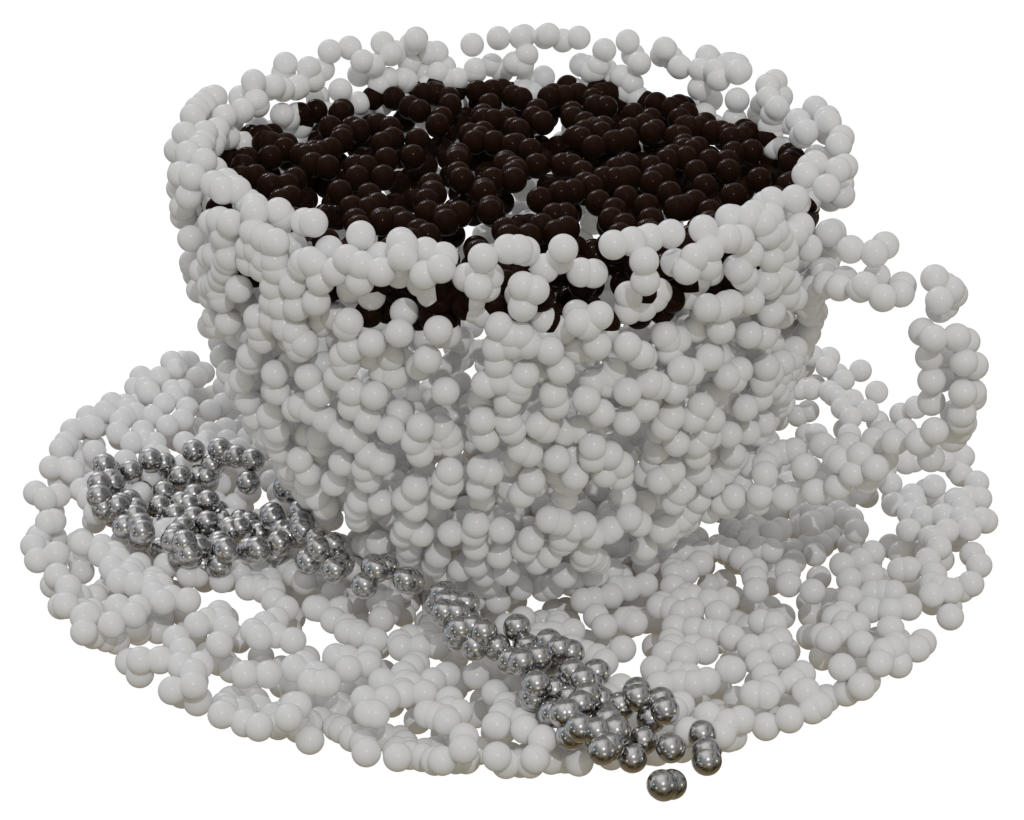
\includegraphics[scale=0.2]{Images/Point Cloud Cup}
	\caption{Point cloud representation of a coffee cup.}
	\label{fig:point_cloud_cup}
\end{figure}

A point cloud is set of unordered 3D coordinates sampled from an object's surface. Point clouds are unstructured and lack topological data~\cite{Xiao2020}. However, this simplicity makes it easy to acquire point clouds using 3D scanning technologies such as Light Detection and Ranging (LIDAR) and photogrammetry~\cite{Leberl2010}. Photogrammetry is an algorithm that uses multiple photos taken from different angles to triangulate points on a surface. Photogrammetry scans are greatly accessible since they can be performed using just a smartphone~\cite{Micheletti2015}.

Despite its accessibility, point clouds did not see use in 3D learning techniques until 2017~\cite{Xiao2020}. Extracting features from point clouds is a challenge since the points are unordered, yet analyzing the proximity between neighboring points is crucial. The points cannot be sorted beforehand because the order would be inconsistent across multiple scans of the same object~\cite{Qi2017}. The 2017 work PointNet~\cite{Qi2017} is the first to tackle this challenge. The PointNet architecture directly extracts features from a point cloud using Multi-Level Perceptrons (MLPs) in order to solve the problems of shape classification and part segmentation. The encoder network is composed of two transform layers, two MLP subnetworks, and a max pooling layer. The transform layers align the features to make the model invariant to rigid transformations such as translation, rotation, and scaling. The first MLP network takes an $n$x3 input matrix containing the coordinates of $n$ points. This network analyzes the neighbors of each point and encodes the local structure features into an $n$x64 vector. The local features are then fed through a second MLP network and a max pooling layer to generate a 1x1024 global feature vector. A max pooling layer was chosen because it is a symmetric function that ignores the permutations of the input points. The shape classification model analyzes just the global features while the part segmentation model analyzes both the local and global features~\cite{Qi2017}. PointNet proved that features can be extracted directly from point clouds and established the foundation for subsequent work.

Follow up work~\cite{Xu2018, Li2018, Wu2019} implements Convolutional Neural Networks (CNNs) instead of MLPs to encode points. While the PointNet architecture has a layer for local features and a layer for global features, CNNs are designed with many feature layers of varying resolution. The increased number of feature layers enables CNN based models to better analyze hierarchical data than MLP based models. As a result, CNN based models surpass PointNet in both shape classification and part segmentation accuracy~\cite{Wu2019}.

Further work~\cite{Fan2017, Achlioptas2018} demonstrates that deep learning models can be trained to generate a point cloud reconstruction of an input. The model presented in~\cite{Fan2017} analyzes a 2D image of an object and generates a cloud of 1024 points to represent its surface. The model is also capable of inferring occluded parts of an input. CNN networks are used for both the image encoder and point cloud decoder. The model in~\cite{Achlioptas2018} uses the PointNet encoder as a base and adds a fully connected MLP decoder network to generate a point cloud. The work experiments with two architectures. The first is an autoencoder network trained using a loss function. The second is a Generative Adversarial Network (GAN) that uses the autoencoder network as a generator alongside an MLP discriminator. Both architectures demonstrate strong results, with the autoencoder slightly outperforming the GAN.

Although point clouds only offer a sparse approximation of a surface, the low-dimensionality proves useful in efficiently learning 3D features.


\subsection{Polygon~Mesh}
\label{subsec:polygon_mesh}

\begin{figure}[ht]
	\centering
	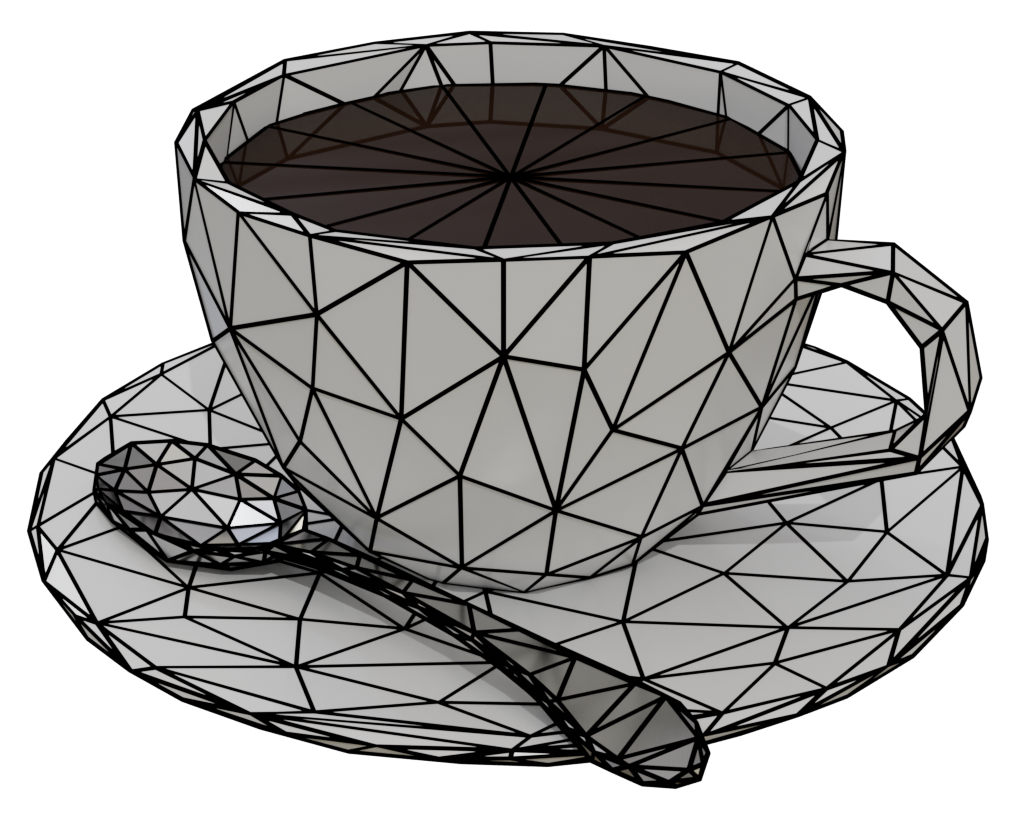
\includegraphics[scale=0.2]{Images/Mesh Cup}
	\caption{Triangle mesh representation of a coffee cup. The black lines depict the connecting edges between vertices.}
	\label{fig:mesh_cup}
\end{figure}

Mesh-based models consist of vertices connected by flat polygonal faces. Unlike point clouds, meshes can represent surface topology and details~\cite{Xiao2020}. Polygon meshes are the most popular 3D representation for use in computer graphics because they can be quickly rendered into images~\cite{Watt1996}. Another unique benefit is that meshes are easy to deform and animate~\cite{Wang2018}. These qualities make mesh-based models ideal for video games, virtual reality, and film~\cite{Nash2020}. One downside is that meshes cannot be directly acquired using 3D scanners. This is circumvented by using surface reconstruction techniques to generate meshes from point cloud scans~\cite{Yuan2022}.

The prevalence of polygon meshes has motivated many mesh-based deep learning models. Since the structure of a polygon mesh is complex, these models adopt unique architectures to simplify the problem. To directly process polygon meshes, models such as FeaStNet~\cite{Verma2018} and MeshCNN~\cite{Hanocka2019} employ Graph Convolutional Networks (GCN). A mesh can be seen as a directed graph of interconnected nodes. This enables graph-based methods such as GCN to directly consume meshes as input. While a traditional CNN applies filters to a group of pixels in an image, a GCN applies filters to a group of nodes or edges in a graph. Like CNNs, GCNs support pooling operations to extract features from a mesh~\cite{Verma2018}. In addition to pooling operations, MeshCNN introduces graph-based unpooling operations to increase the resolution of a mesh.

Techniques to generate meshes are more varied. AtlasNet~\cite{Groueix2018} employs an MLP to reconstruct a point cloud using multiple mesh patches. The model starts with flat planes as a template. The planes are then deformed and stitched together to represent the surface of the point cloud. This papier-m{\^a}ch{\'e} approach is efficient but does not produce a continuous surface~\cite{Groueix2018}. Pixel2Mesh~\cite{Wang2018} and Point2Mesh~\cite{Hanocka2020} both deform a 3D template mesh through cascaded refinement to represent the input. Instead of a flat plane, Pixel2Mesh and Point2Mesh start with a sphere encompassing a point cloud. The template is then deformed in a coarse-to-fine manner with the resolution of the template mesh increasing each iteration. Starting with a lower resolution allows the model to quickly build a rough approximation of the shape. Then the resolution is gradually increased to allow for more fine adjustments. Working with the minimum required resolution for any given iteration greatly improves the efficiency of these models. Unlike AtlasNet, Pixel2Mesh and Point2Mesh are guaranteed to generate manifold surfaces since the initial shape template is manifold. A limitation of current deformation based models is their inability to represent arbitrary topologies. Models with no means to merge or remove geometry cannot create holes in the template mesh~\cite{Wang2018, Hanocka2020}.

\newpage

PolyGen~\cite{Nash2020} takes the most direct approach in generating 3D meshes. A vertex generation network predicts a variable number of vertices to represent the input. The vertices are then fed to a face generation network that best connects the vertices with edges and faces. Both networks are implemented as transformers~\cite{Nash2020}. Similar to a Long Short-Term Memory (LSTM) network or a Recurrent Neural Network (RNN), a transformer consumes and produces sequential data. However unlike  an RNN or LSTM, the innovative architecture of a transformer network allows the outputs to be computed in parallel. This not only makes training and running the network faster, but also enables longer input and output sequences~\cite{Vaswani2017}. Transformers have a fixed output size, so the authors include a stopping token to the output parameters of the vertex network to allow for variable size meshes. The maximum resolution of the output mesh is 1200 vertices and 800 faces. Because PolyGen directly generates meshes, it can represent geometric shapes with far fewer polygons than competing models. The biggest limitation of PolyGen is its small output resolution. The computational cost of a transformer network increases quadratically with the size of the network. Despite some optimizations, the transformer networks are too inefficient at scale to generate more detailed meshes. Due to this limitation, PolyGen is focused on representing simple geometric shapes using the minimum number of polygons~\cite{Nash2020}.

The polygon mesh is one of the most convenient 3D formats. However, deep learning models struggle to generate meshes due to their non-Euclidean nature. Existing models are either limited in output detail or suffer from a small output resolution.

\newpage


\subsection{Occupancy~Grid}
\label{subsec:occupancy_grid}

\begin{figure}[ht]
	\centering
	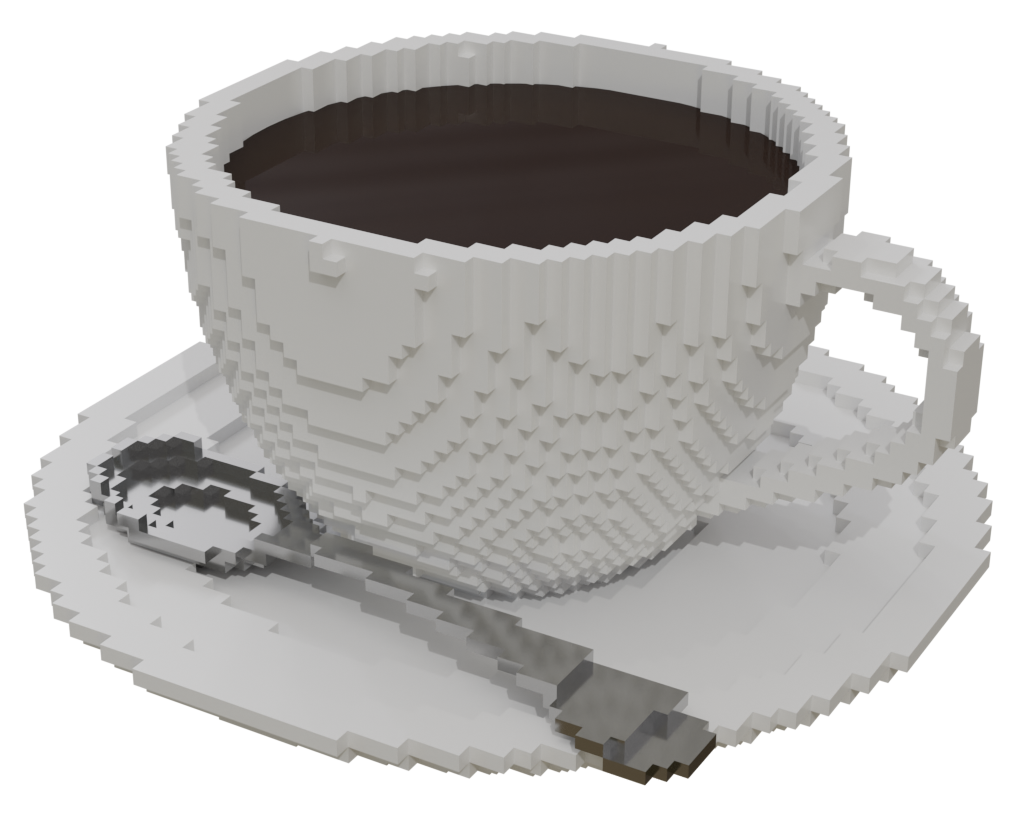
\includegraphics[scale=0.2]{Images/Voxel Cup}
	\caption{Voxel grid representation of a coffee cup.}
	\label{fig:voxel_cup}
\end{figure}

An occupancy grid, also known as a voxel grid, discretizes 3D space into a regular grid of voxels. Each voxel stores a probability that it is occupied or vacant. A volume represented by a set of occupied voxels is called an occupancy map. There are several occupancy grid variations that store different values in the voxels. A binary occupancy grid stores binary occupancy values in the voxels instead probabilities~\cite{Konolige1997}. Some variations also add a parameter for voxels with an unknown state~\cite{Ahmed2018}.

The first work to apply occupancy grids in deep learning is 3D ShapeNets~\cite{Wu2015}. The ShapeNets model takes a four-channel RGB-D image as input. In addition to red, greed, and blue color values, RGB-D images store the distance from the camera to the scene in each pixel. The RGB-D images are converted to an occupancy map as a pre-processing step. The input occupancy map dimensions are $30^3$ voxels with 3 voxels of padding on all sides of the object. Parts of the scene are occluded in a single-view RGB-D image. To accommodate for this, the authors add a third ``occluded'' state to each voxel in addition to the ``vacant'' and ``occupied'' states~\cite{Wu2015}.

The voxel representation is then fed into a modified Deep Belief Network (DBN) that the authors call a Convolutional Deep Belief Network (CDBN)~\cite{Wu2015}. DBNs offer several advantages over traditional neural networks, including more efficient learning and the ability to pre-train on unlabeled datasets. A DBN is composed of multiple Restricted Boltzmann Machines (RBMs) that are stacked such that the hidden layer of one RBM becomes the visible layer of the next~\cite{Aljabery2020}. Each RBM layer is trained to represent the data in the previous layer. Earlier RMBs learn low level features while later RBMs learn high level features. The features encoded in the last layer of the DBN can then be decoded using other machine learning techniques~\cite{McAfee2008}. The ShapeNets CDBN architecture adds convolution operations to a standard DBN to make it compatible with 3D inputs. The ShapeNets model was trained using contrastive divergence for unsupervised pre-training and a method similar to the wake-sleep algorithm for supervised fine-tuning. The resulting feature vector is then fed to a Support Vector Machine (SVM) to perform shape classification~\cite{Wu2015}.

VoxNet~\cite{Maturana2015} improves upon ShapeNet with a 3D CNN architecture. It simple in theory to extend a 2D image processing CNN to handle 3D occupancy grids. In practice, however, the increased memory and computational requirements added by the extra spatial dimension pose a challenge. Due to these restrictions, the VoxNet architecture limits the input size to a grid of $32^3$ voxels. The voxel input is fed through a network consisting of two convolution layers, one pooling layer, and two fully-connected layers to produce class label predictions. To better capture fine details, VoxNet implements a multiresolution architecture by combining two of these convolutional networks. The networks are identical but are fed different inputs. Each voxel in the coarse input represents a volume of $0.2\text{m}^3$ while the each voxel of the fine input represent $0.1\text{m}^3$. Both inputs share the same dimensions but the coarse input captures a larger volume than the fine input. The outputs of both networks are then combined to produce a final class prediction. The VoxNet architecture is easier to train than ShapeNet since it contains ten times fewer parameters. VoxNet also outperforms ShapeNet in classification accuracy~\cite{Maturana2015}.

Seeing as the main drawback of occupancy grids is the high computational demand, several works focus on optimization. The authors of LightNet~\cite{Ye2016} optimize using a multi-task learning approach. This is a technique where a single model is trained to solve multiple tasks at once. In doing so, the model avoids overfitting and learns to extract general features. In the case of LightNet, the model is trained to predict the shape class and orientation of an input occupancy map. LightNet enjoys performance improvements over VoxNet but is still constrained to an input resolution of $32^3$ voxels~\cite{Ye2016}. 

Instead of optimizing the model directly, Octree Generating Networks (OGN)~\cite{Tatarchenko2017} optimize the data format. The methods discussed thus far store each voxel of the occupancy grid in a dense array. Continuous arrays are simple to work with but have increased dimensionality because they store redundant data. OGN compresses the input occupancy grid using an octree data structure. The root node contains 8 octants encompassing the entire volume. Each of the 8 octants is a child node that either subdivides the volume into a further 8 octants or terminates in a leaf node. This spacial partitioning scheme efficiently summarizes groups of similar voxels and reduces the format size. The octree format is used for both the input and output of the OGN architecture. OGN is a self-supervised convolutional autoencoder network trained to reconstruct an input occupancy map. The data compression enables a massive jump in resolution to $512^3$ voxels on consumer hardware. A downside to this approach is the complexity needed to support octrees. The octree structure is stored in a hash table for quick lookup. If this hash table is not available during runtime, the performance of the model significantly decreases. And despite the large optimization, OGN can take over a week to train at higher resolutions~\cite{Tatarchenko2017}.

Occupancy grids provide rich volumetric data for object classification and reconstruction tasks. While prior works implement occupancy map representations to great success, the computational cost limits their applications.

\newpage


\subsection{2D Projection}

\begin{figure}[ht]
	\centering
	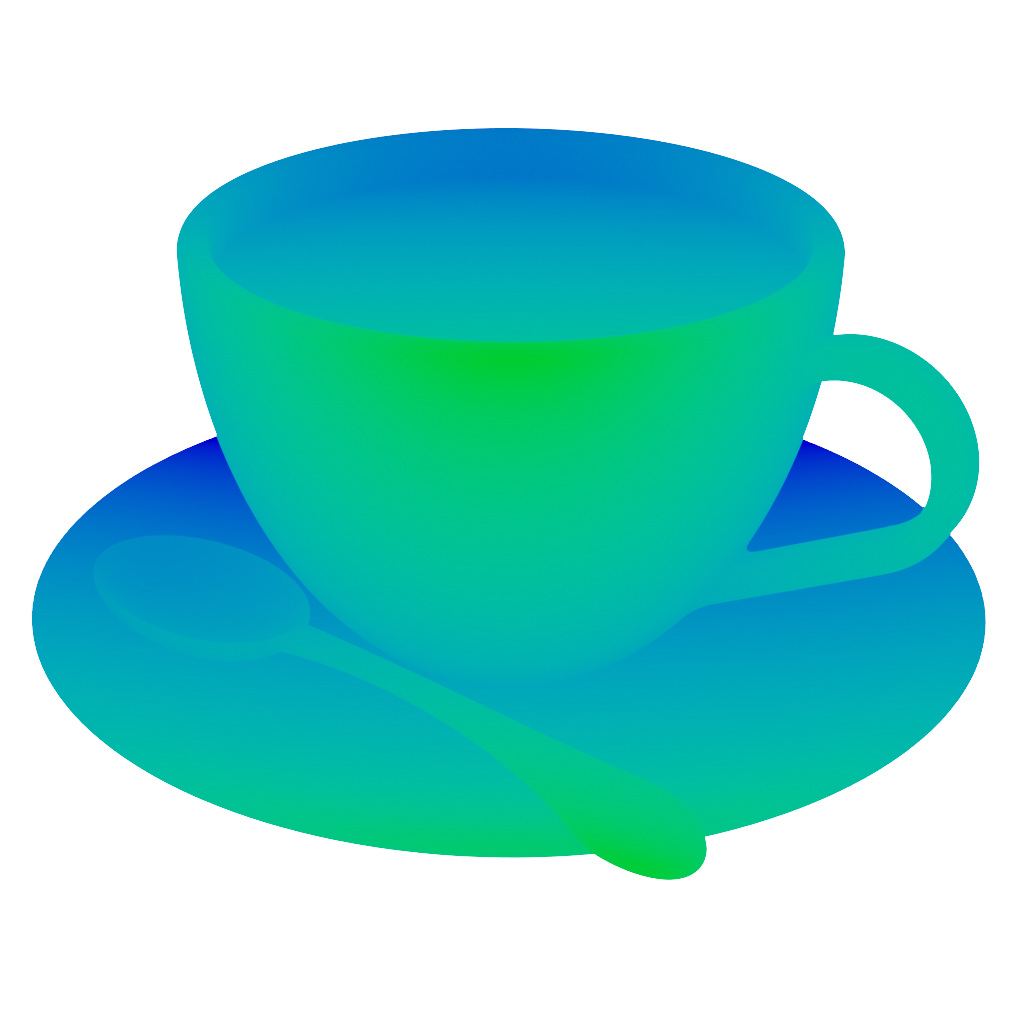
\includegraphics[scale=0.2]{Images/Depth Map Cup}
	\caption{Depth map representation of a coffee cup. Points closer to the camera are colored green and points further from the camera are colored blue.}
	\label{fig:depth_map_cup}
\end{figure}

A 3D object can be projected onto a 2D image while maintaining key features for computer vision tasks. Removing a spacial dimension reduces the computational requirements and improves efficiency. The downside is that useful features are lost in the projection. Different types of projections have varying levels of accessibility and feature quality~\cite{Ahmed2018}.

The most common projection is an RGB image, which can be captured using a digital camera or by rendering a 3D model. Prior work~\cite{Zhu2014, Su2015, Choy2016, Smith2018} uses CNNs to extract features from a sequence of multi-view RGB images. Processing multiple viewpoints of an object provides additional context that is missing from a single view. The extracted features are descriptive enough for use in object classification and reconstruction tasks. The caveat is that the an additional encoder network is needed for each input image. Using more images provides more information but increases the model complexity. Further work~\cite{Fan2017, Wang2018, Niu2018, Genova2020, Pan2019} manages to complete the same tasks using only one single-view image. Requiring only one input image makes the model more accessible since multiple viewpoints are not always available. The model complexity increases, however, to compensate for the missing features. A single-view encoder network must be invariant to the orientation of the image and perform the same analysis using fewer features. Instead of multiple images, \cite{Shi2015, Sfikas2017, Cao2017} use panoramic images to capture an object from all sides. The models in~\cite{Shi2015, Sfikas2017} project the object onto a cylinder while the model in~\cite{Cao2017} projects onto a sphere. Panoramic images encode the same features as a sequence of multi-view images but in a more compact format. The models in~\cite{Zhu2014, Genova2020, Shi2015, Sfikas2017, Cao2017} operate on depth maps, which capture depth information instead of color. Each pixel of a depth map encodes the distance from the camera to the surface of the subject. Depth maps provide more spacial information than an RGB image but omits any lighting, color, or texture information.

The application of 2D projections is not limited to feature extraction. SurfNet~\cite{Sinha2017} demonstrates that a generative model can be trained to synthesize 2D projections of 3D objects. It is then trivial to convert the 2D projection back into a 3D object. SurfNet represents shapes using what the authors call a geometry image. Geometry images use an area-preserving spherical projection to capture shapes. Instead of color or depth information, geometry images store the 3D coordinate of each point represented in the image. This format provides rich geometric information while keeping compatibility with traditional CNNs~\cite{Sinha2017}.

A 2D projection provides a simple yet powerful representation for real-time applications. The main limitation is that the details of complex shapes are lost. Additionally, current works can only represent manifold and continuous surfaces containing no holes~\cite{Sinha2017}.

\newpage


\subsection{Implicit~Surface}
\label{subsec:implicit_surface}

\begin{figure}[ht]
	\centering
	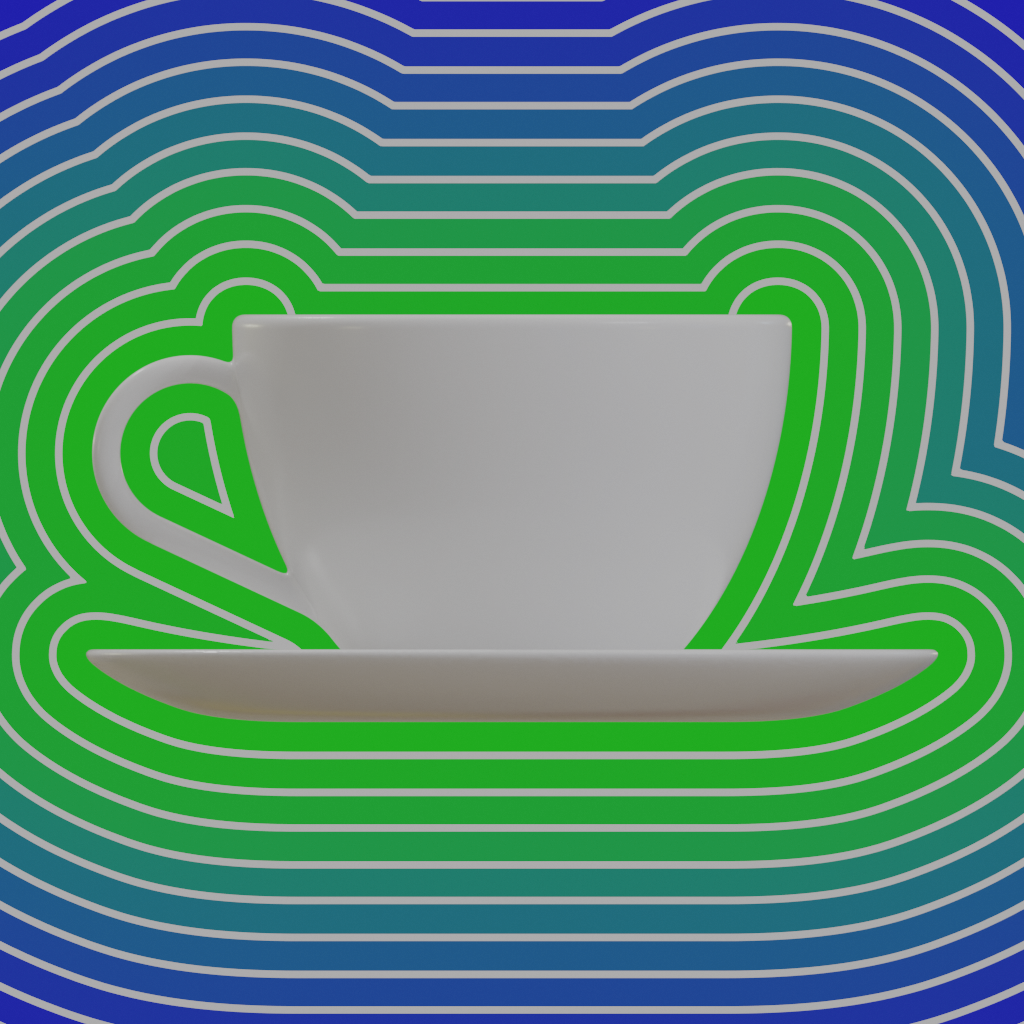
\includegraphics[scale=0.2]{Images/SDF Cup}
	\caption{Visualization of an SDF representing a coffee cup. Points closer to the surface are colored green and points farther from the surface are colored blue. Each white isoline consists of points that are equidistant from the surface.}
	\label{fig:sdf_cup}
\end{figure}

Implicit surface representations have become a popular research topic in recent years. Neural networks can be trained to learn a function that implicitly defines a surface. Since the surfaces are implicit, they require relatively little memory and have no maximum resolution~\cite{Xiao2020}.

The 2019 work DeepSDF~\cite{Park2019} popularized the use of implicit surfaces for deep 3D learning. The DeepSDF network is trained to learn the SDF function for a specific input shape. Given a query point, the network predicts the distance from the query point to the surface of the represented shape. DeepSDF is implemented using only a decoder network without an accompanying encoder. The authors describe this architecture as an autodecoder. The motivation to use an autodecoder originates from ITNet~\cite{Tan1995}, which demonstrates that a decoder network can be effectively trained on its own. In addition to being faster to train, an autodecoder network can generalize better than an autoencoder. The DeepSDF autodecoder is an MLP network that takes a latent vector and query point as input and outputs a distance value. The architecture needs to be trained in two phases. The first phase is aimed at training the parameters of the MLP decoder on a class of shapes. The dataset consists of query point and expected SDF value pairs for many shapes of the same class. Since there is no encoder network, the latent vector must also be trained for each input shape. The latent vector is initialized with random values for each new shape the network is trained on. The second phase trains the network to represent a  input shape not present in the training dataset. The parameters of the decoder are held constant while the values of the latent vector are optimized. DeepSDF is fast to train and can produce detailed representations of complex geometry. The autodecoder architecture allows DeepSDF to accurately infer missing geometry and interpolate between latent vectors. The trained model is compact and can be easily incorporated into other applications. The main disadvantage is that DeepSDF is a black box solution that cannot be modified once trained~\cite{Park2019}.

Several papers have extended the work of DeepSDF. In~\cite{Gropp2020}, a novel loss function is used to achieve higher fidelity reconstructions. DISN~\cite{Wang2019} modifies the DeepSDF architecture by adding a separate MLP network to encode the query point. And \cite{Kleineberg2020} implements DeepSDF as a progressively growing GAN architecture. The authors experiment with two types of discriminator network. A 3D CNN network is used for the occupancy map discriminator and PointNet is used for the point cloud discriminator. The original DeepSDF decoder network is used as the generator. The resolution of the model is lowest at the start of training. As training progresses, new layers are added to the generator and discriminator networks to increase their resolution. Progressively growing the model resolution helps the model learn faster than starting with a high resolution model~\cite{Kleineberg2020}.

Research has also been conducted on implicit surfaces other than SDFs. Several recent works~\cite{Mescheder2019, Peng2020} train a model to learn an occupancy function. Where an occupancy grid stores the occupancy value for a fixed number of voxels, an occupancy function returns the occupancy value for any given query point. Like an SDF, an occupancy function is an implicit representation with no maximum resolution. The OccNet~\cite{Mescheder2019} architecture relies on existing 3D encoders to extract features from an input shape. The shape features and a set of $n$ query points are fed to a 5-layer CNN. Then the CNN predicts the occupancy value for each of the $n$ points. Accepting multiple query points allows the model to be efficiently trained and run in parallel~\cite{Mescheder2019}. The model in~\cite{Peng2020} uses PointNet to encode features for each point of an input point cloud. The features are then projected onto a discretized 2D or 3D grid. A feature vector is created for a query point by interpolating the features for the closest points on the feature grid. Finally, the query point and the interpolated feature vector are processed by an MLP to produce an occupancy value~\cite{Peng2020}.

Not all techniques involve learning an implicit surface directly. The model presented in \cite{Zheng2021} learns to deform an input shape to fit a learned template. The model is trained on a single class of shape, such as chairs. An MLP network learns the SDF of a template that captures the common features of all the chair samples. To represent a specific input chair, an LSTM network produces a set of deformations that transforms the input chair onto the template. Then any SDF queries for an input chair can be transformed into the template space to produce an accurate distance value. Using a common template makes learning new samples faster. The disadvantage is that samples deviating too far from the learned template cannot be accurately represented~\cite{Zheng2021}.

Implicit surfaces are memory efficient, detailed, and have no resolution limit. They can be learned efficiently using relatively simple architectures. The main limitation is that the model itself becomes the 3D representation. Once learned, the implicit surface cannot be modified. Algorithms such as Marching Cubes~\cite{Lorensen1987} can be used to convert the implicit surface to a high-resolution polygon mesh~\cite{Xiao2020}. Doing so, however, removes the memory efficiency and limitless resolution of the implicit representation.

\newpage


\subsection{Structured~Representation}
\label{subsec:structured_representation}

\begin{figure}[ht]
	\centering
	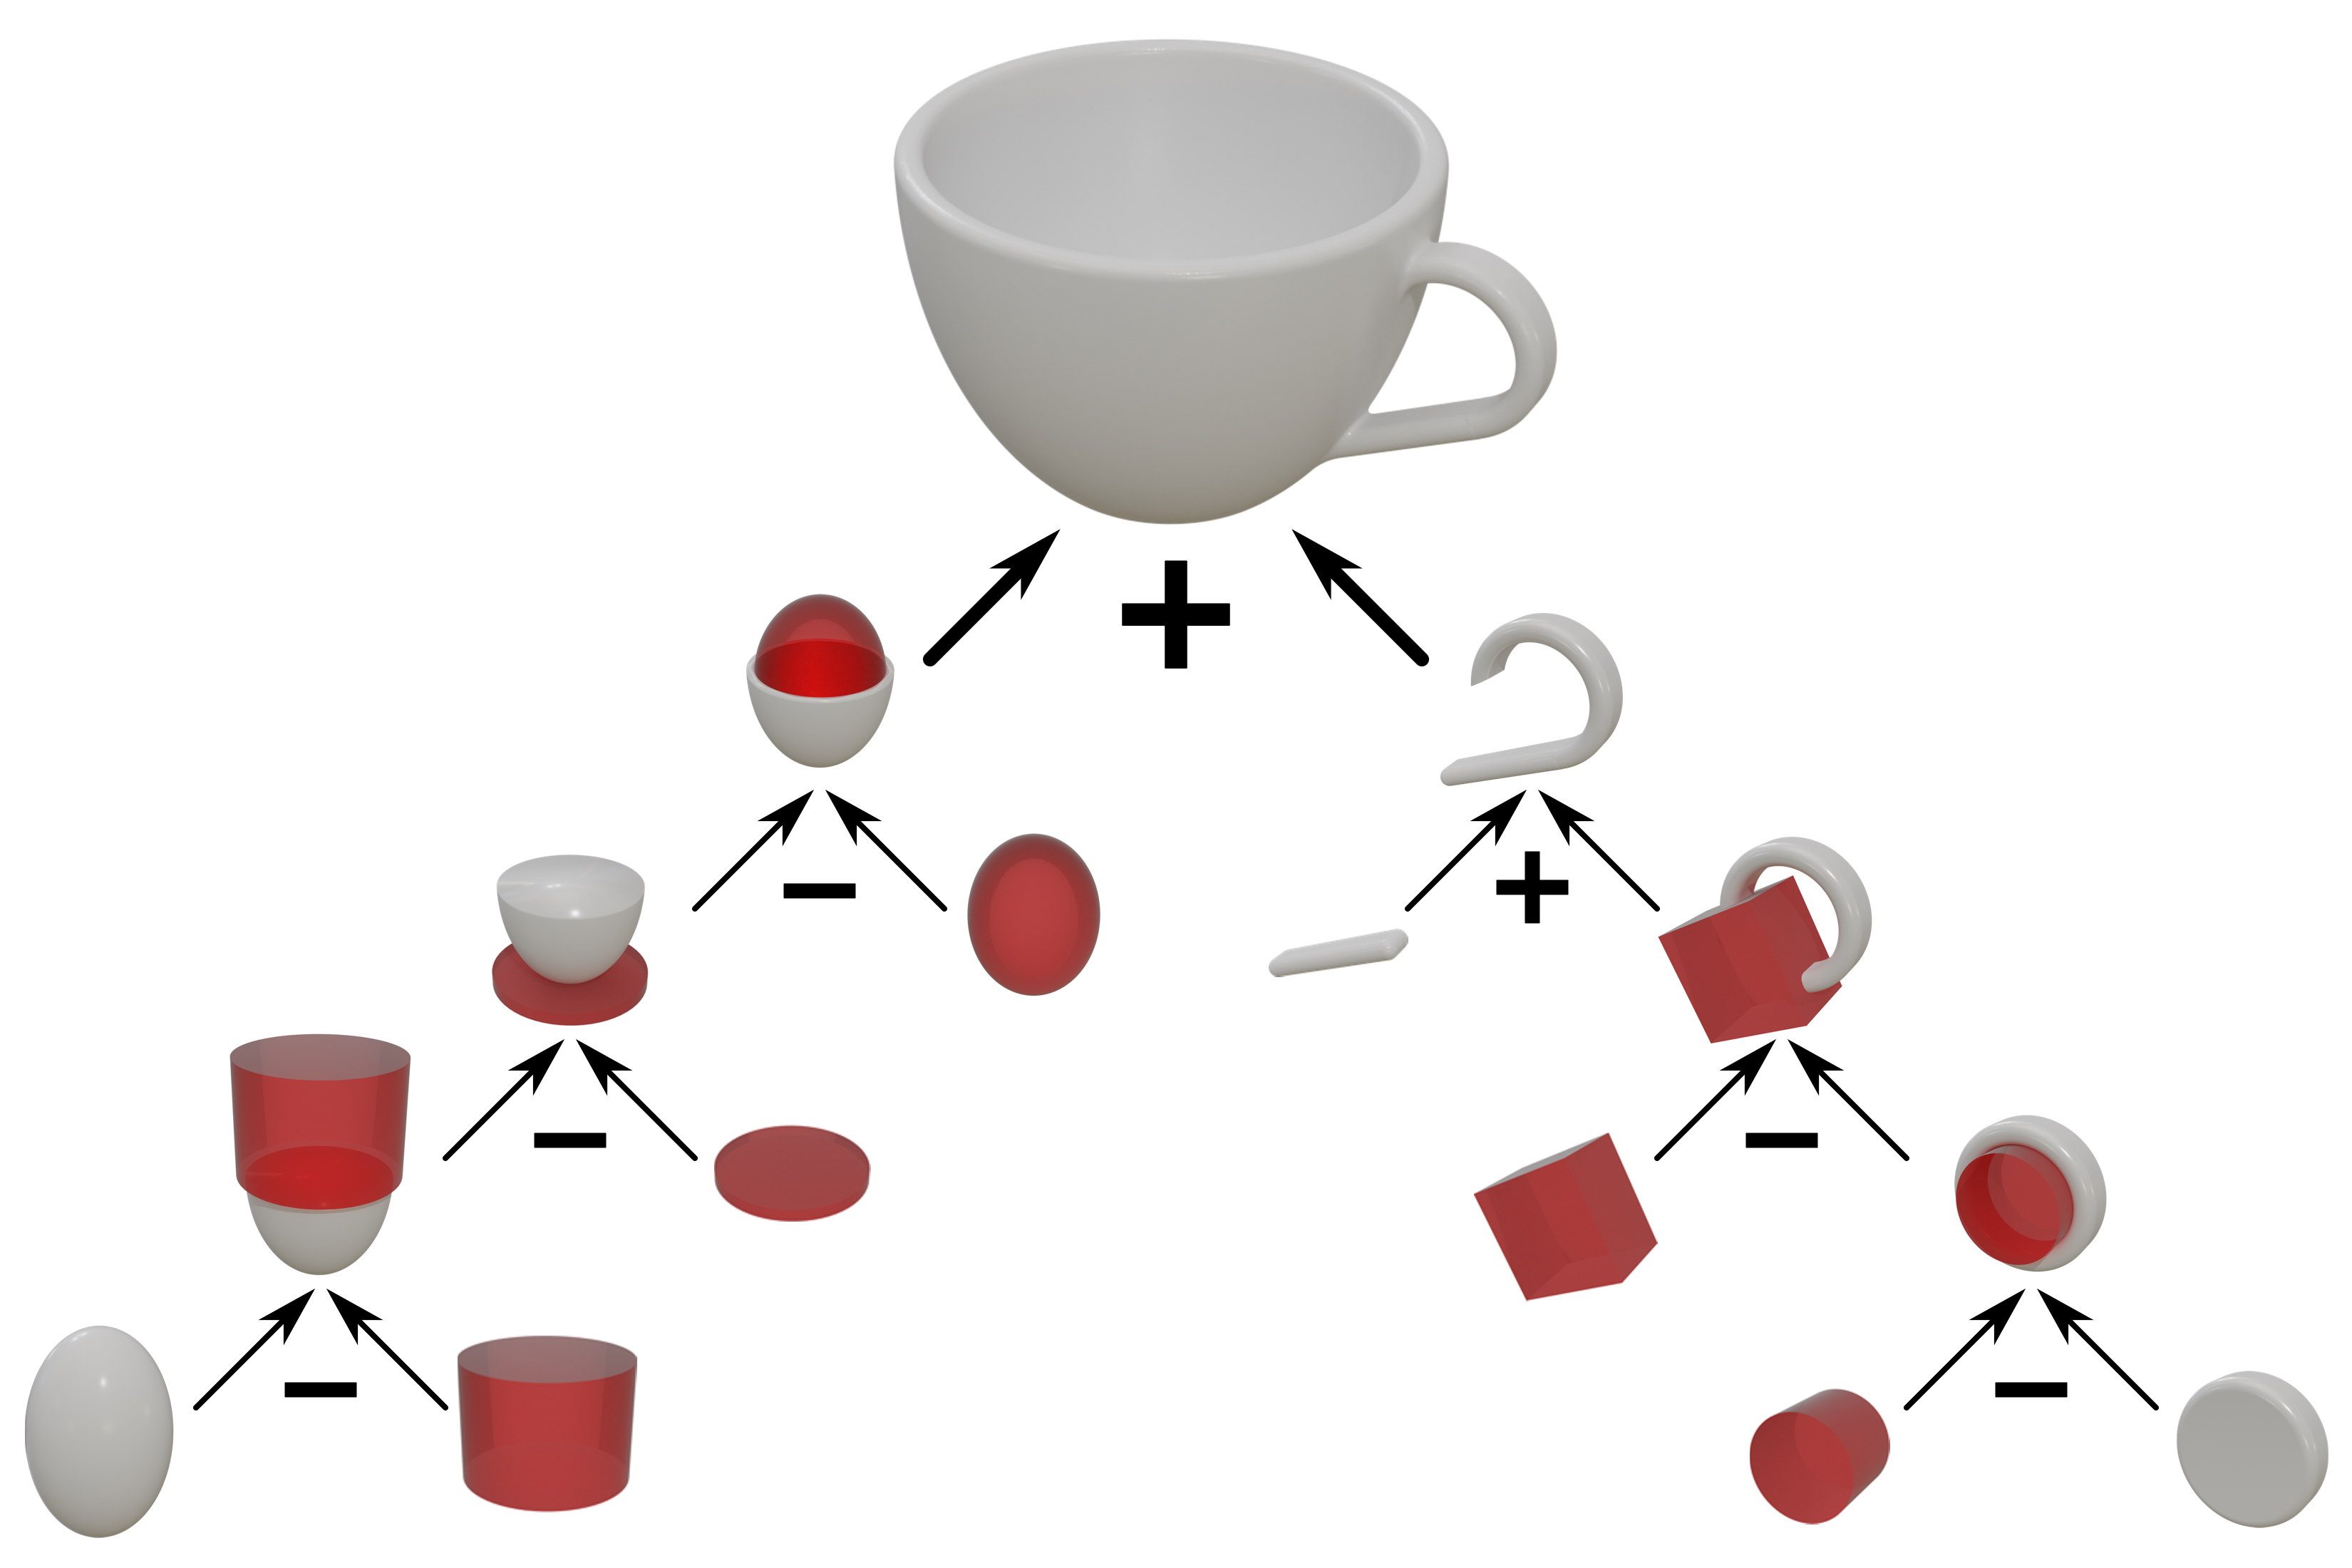
\includegraphics[scale=0.5]{Images/CSG Cup}
	\caption{The CSG tree of a coffee cup. The leaves of the tree are SDF primitives which are combined through union (+) and subtract (-) operations. The primitives being subtracted are colored red.}
	\label{fig:csg_cup}
\end{figure}

Both natural and man-made objects are highly structural. Repeating patterns and symmetries appear within individual objects and between objects of the same class. Learning an object's structure can help in better understanding the object and concisely describing its shape. To this end, recent work has experimented with training neural networks to learn structured representations of 3D objects~\cite{Tulsiani2017}.

Early attempts represented object structure using a collection of oriented cuboid primitives. The architecture in~\cite{Tulsiani2017} uses a 3D CNN to encode an occupancy map. Then two fully connected layers predict up to 20 cuboids to reconstruct the input. The model is trained without supervision using a loss function. The loss measures reconstruction accuracy and encourages the model to minimize the number of cuboids it uses~\cite{Tulsiani2017}. 3D-PRNN~\cite{Zou2017} uses a supervised learning approach. To generate a synthetic dataset, the authors develop an algorithm to parse a cuboid structure from point clouds. The cuboids are then rendered into depth maps and fed to a CNN encoder. An LSTM and Mixed Density Network (MDN) are used to sequentially predict cuboid primitives. The MDN is a fully connected layer that predicts the mean, standard deviation, weight, and correlation for each parameter of the output primitive. Training is driven by the loss between the predicted structure and synthesized ground truth structure~\cite{Zou2017}. Learning simple cuboid structures allows these methods to recognize different parts of an object. Cuboids alone, however, are not expressive enough to accurately reconstruct the input objects.

The structure of complex objects can be better described by using a variety of shapes primitives. The model in~\cite{Li2019} predicts object structures using four primitives: planes, spheres, cylinders, and cones. A version of the PointNet encoder is used to predict which primitives encompass which points of an input point cloud. These features are then processed by hand-crafted primitive fitting functions to determine the orientation and scale of each primitive. The model is trained on a dataset of Computer Aided Design (CAD) models primarily composed of planes, spheres, cylinders and cones. The model is trained end-to-end under the supervision of the CAD dataset~\cite{Li2019}. While effective in predicting simple object structures, primitive fitting methods are ultimately limited by their selection of primitives.

The challenge of limited primitive selection is solved using parameterized primitives that represent an unlimited number shapes. The models in both~\cite{Paschalidou2019} and~\cite{Paschalidou2020} reconstructs objects using superquadrics. This is a function that can represent cuboids, spheres, cylinders, and everything in between. Both models use the loss between the input and the reconstruction to self-supervise training. These models prove that using superquadrics significantly improves accuracy over using cuboids~\cite{Paschalidou2019}. Even better accuracies can achieved using more versatile primitives. CvxNet~\cite{Deng2020} uses convex polytopes, or simply convexes, as primitives. A convex is defined as the volume encompassed by a collection of hyperplanes. CvxNet is trained to predict the normal vector and position of the hyperplanes that define each primitive shape. Convexes are simple and can express any basic convex shape. But convexes are inefficient at modeling geometry with concavities~\cite{Deng2020}. This limitation does not apply to the neural primitives introduced in~\cite{Paschalidou2021}. The neural parts model uses MLP networks to predict a homeomorphic mapping that transforms a sphere into any target shape. The loss function includes a coverage loss that ensures each neural primitive contributes equally to the reconstruction. Using more primitives results in simple shapes that capture local structures. And using fewer primitives results in complex shapes that represent high-level structures. The ability to capture structures with varying levels of abstraction is useful for meeting the needs of different applications. And the neural parts model can extract these structure while achieving high reconstruction accuracy~\cite{Paschalidou2021}. The implicitly defined primitives used in these models share the same advantages and disadvantages as the implicit surface representations discussed in the previous chapter. While expressive and compact, parameterized primitives are difficult to modify once generated.

CSG representations offer a compromise between the simplicity of non-deformable primitives and the accuracy of deformable primitives. Despite using the same simplistic primitives as~\cite{Li2019}, CSG representations can represent concavities and achieve higher reconstruction accuracy by using boolean operations. CSG models are unable to parse structures with the same level of abstraction as methods like~\cite{Paschalidou2021} that use fewer, more descriptive primitives. But the simplicity of CSG models allow them to be more compact and modifiable~\cite{Paschalidou2021}.

CSGNet~\cite{Sharma2018} is the first work to apply machine learning to CSG reconstruction. The authors experiment with both 2D and 3D CSG reconstruction as well as different training methods. The 2D architecture encodes a 64x64 1-bit image using a CNN and predicts a CSG program using a GRU decoder. The 3D architecture encodes a $64^3$ voxel input using a 3D CNN and uses a similar GRU decoder. The GRU decoders generate seven commands to form a CSG program. There are thee types of command. The first adds a primitive to the reconstruction. The second applies a boolean operation to the previous two primitives. And the third marks the end of the program. The authors generate synthetic 2D and 3D datasets by randomly applying primitives and boolean operations. The CSG programs are then discretized into images and voxel grids for the 2D and 3D datasets respectively. The 2D dataset consists of circle, square, and equilateral triangle primitives while the 3D dataset consists of sphere, cube, and cylinder primitives. The primitives can be positioned and scaled but not rotated. Instead of parameterizing the primitives, the authors encode each combination of shape, position, and scale as a unique primitive. The 2D dataset contains a total of 396 unique primitives. Including the 3 boolean operators and the stop command, there are 400 possible commands. Similarly, the 3D dataset has 6631 unique primitives and 6635 possible commands. Each GRU decoder unit predicts the most likely command through a one-hot vector of all available commands. The decoder also implements beam search to improve accuracy. The network can be trained using both supervision from the ground truth samples and unsupervised reinforcement learning driven by reconstruction accuracy. Training exclusively using reinforcement learning did not produce good results, so the authors use it as a refinement step after supervised pre-training. The authors also develop a heuristic algorithm to adjust the positions of the output primitives to further improve accuracy. The nearest neighbor algorithm is used as a performance baseline, which retrieves the CSG program from the training dataset that best represents the test sample. The full CSGNet implementation with reinforcement learning tuning, a beam width of 10, and the heuristic adjustment algorithm shows a marked improvement over the nearest neighbor algorithm. But the model accuracy is far worse than alternate solutions. CSGNet succeeds as proof of concept demonstrating CSG can be used successfully in deep learning. It fails as a practical solution to object recognition and reconstruction tasks~\cite{Sharma2018}.

UCSG-Net~\cite{Kania2020} expands upon the work of CSGNet with an improved architecture. UCSG-Net is a fully unsupervised model that is more flexible and accurate than CSG-Net. Like CSGNet, UCSG-Net uses either a 2D or 3D convolutional network to encode images or occupancy maps respectively. Unlike CSGNet, the UCSG-Net decoder uses three layers to generate a CSG representation. The primitive parameter prediction layer is an MLP network that predicts the shape, scale, position, and rotation for a fixed number of SDF primitives. The SDF-To-Indicator function layer classifies distances sampled from the SDF primitives as binary occupancy values. Lastly, multiple CSG layers are implemented by GRU networks to apply boolean operations to the predicted primitives and build a CSG representation. The model is trained by minimizing the the mean squared error reconstruction loss between the occupancy values of the predicted CSG model and the ground truth mesh. The continuous parameters of the UCSG-Net primitives allow for significantly finer control than the discretized parameters of the CSG-Net primitives. And the fully unsupervised end-to-end training scheme allows UCSG-Net to train on large, unlabeled datasets of real world objects~\cite{Kania2020}. Despite the improvements, UCSG-Net is still limited in reconstruction accuracy. The authors experimented with a maximum of 5 CSG layers in the paper. A CSG tree of this depth fails to represent intricate shapes. And the architecture is too inefficient to support more CSG layers~\cite{Ren2021}.

Unlike CSGNet or UCSG-Net, CSG-Stump is optimized to handle large CSG trees. The DGCNN~\cite{Phan2018} convolutional encoder network is borrowed to extract features from a point cloud input. The features are then processed by a dual-headed decoder. The primitive head uses an MLP to predict the size, position, and rotation for an equal number of box, sphere, cylinder, and cone primitives. Independently from the primitive head, the connection head predicts which boolean operations to apply to which shapes. A single layer perceptron is used for each of the three boolean operations: complement, intersect, and union. Each perceptron outputs a binary connection matrix indicating which shapes the boolean operation should be applied to. The outputs of the primitive head are converted from SDFs to binary occupancy functions using the sigmoid function. Finally, the CSG-Stump constructor takes both the predicted primitives and the three connection matrices to compute the occupancy value for a given query point. Similar to UCSG-Net, the mean squared error reconstruction loss is used to drive the unsupervised training of CSG-Stump. CSG-Stump offers an improvement in maximum primitives and reconstruction accuracy over UCSG-Net. However, CSG-Stump is still limited compared to models using alternate representations~\cite{Phan2018}.

\newpage

\section{Representation~Learning~Architectures}
\label{sec:representation_learning_architectures}

Test

\subsection{Generative~Adversarial~Network}
\label{subsec:generative_adversarial_networks}

Test

\subsection{Autoencoder}
\label{subsec:autoencoders}

Test

\subsection{Cascaded~Refinement}
\label{subsec:cascaded_refinement}

Test